\documentclass[11pt,letterpaper]{article}
\usepackage[lmargin=1in,rmargin=1in,tmargin=1in,bmargin=1in]{geometry}
\usepackage{../style/homework}
\usepackage{../style/commands}
\setbool{quotetype}{false} % True: Side; False: Under
\setbool{hideans}{false} % Student: True; Instructor: False

% -------------------
% Content
% -------------------
\begin{document}

\homework{4: Due 01/07}{Sometimes I get so bored I just want to scream, and then sometimes I actually do scream. I just sort of feel out what the situation calls for.}{Kelly Kapoor, The Office}

% Problem 1
\problem{10} Determine if the relations $f(x)$ and $g(x)$ shown below are functions. Explain why or why not. 
	\[
	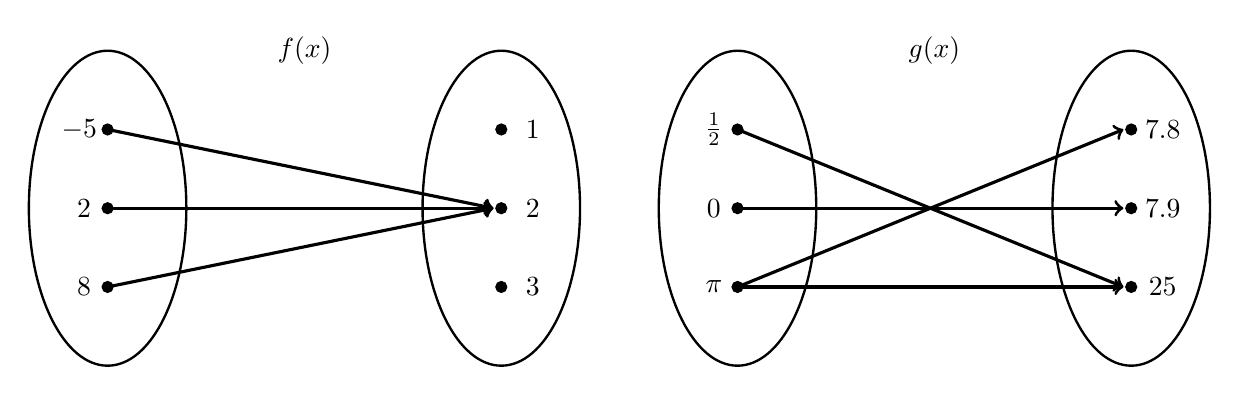
\begin{tikzpicture}
	\node at (2.5,2) {$f(x)$};
	% Ellipses
	\draw[line width=0.03cm] (0,0) circle (1 and 2);
	\draw[line width=0.03cm] (5,0) circle (1 and 2);
	
	% Nodes
	\draw[fill=black] (0,1) circle (0.07);
	\draw[fill=black] (0,0) circle (0.07);
	\draw[fill=black] (0,-1) circle (0.07);
	
	\draw[fill=black] (5,1) circle (0.07);
	\draw[fill=black] (5,0) circle (0.07);
	\draw[fill=black] (5,-1) circle (0.07);
	
	% Arrow
	\draw[line width=0.04cm,->] (0,1) -- (4.9,0);
	\draw[line width=0.04cm,->] (0,0) -- (4.9,0);
	\draw[line width=0.04cm,->] (0,-1) -- (4.9,0);
	
	% Labels
	\node at (-0.3,1) {$\!\!-5$};
	\node at (-0.3,0) {$2$};
	\node at (-0.3,-1) {$8$};
	
	\node at (5.4,1) {$1$};
	\node at (5.4,0) {$2$};
	\node at (5.4,-1) {$3$};
	
	\tikzset{shift={(8,0)}}
	%
	\node at (2.5,2) {$g(x)$};
	% Ellipses
	\draw[line width=0.03cm] (0,0) circle (1 and 2);
	\draw[line width=0.03cm] (5,0) circle (1 and 2);
	
	% Nodes
	\draw[fill=black] (0,1) circle (0.07);
	\draw[fill=black] (0,0) circle (0.07);
	\draw[fill=black] (0,-1) circle (0.07);
	
	\draw[fill=black] (5,1) circle (0.07);
	\draw[fill=black] (5,0) circle (0.07);
	\draw[fill=black] (5,-1) circle (0.07);
	
	% Arrow
	\draw[line width=0.04cm,->] (0,1) -- (4.9,-1);
	\draw[line width=0.04cm,->] (0,0) -- (4.9,0);
	\draw[line width=0.04cm,->] (0,-1) -- (4.9,1);
	\draw[line width=0.04cm,->] (0,-1) -- (4.9,-1);
	
	% Labels
	\node at (-0.3,1) {$\frac{1}{2}$};
	\node at (-0.3,0) {$0$};
	\node at (-0.3,-1) {$\pi$};
	
	\node at (5.4,1) {$7.8$};
	\node at (5.4,0) {$7.9$};
	\node at (5.4,-1) {$25$};
	\end{tikzpicture}
	\] \pspace

\sol The relation $f(x)$ is a function because for each input, there is a unique output. Specifically, we know that $f(-5)= 2$, $f(2)= 2$, and $f(8)= 2$; that is, $f(x)$ is the constant function with output 2. \pspace

The relation $g(x)$ is not a function because there are inputs which have more than one possible output. While we know that $g(\frac{1}{2})= 25$, $g(0)= 7.9$, we do not know $g(\pi)$. We could either have $g(\pi)= 7.8$ or $g(\pi)= 25$. Therefore, this relation is not a function because $g(\pi)$ is not well defined. 



\newpage



% Problem 2
\problem{10} Determine if the relations $f(x)$ and $g(x)$ shown below are functions. Explain why or why not. 
	\begin{table}[!ht]
	\centering
	\begin{tabular}{c|rcc|r}
	$x$ & $f(x)$ & \hspace{1cm} & $x$ & $g(x)$ \\ \cline{1-2} \cline{4-5}
	$1$ & $5$ & & $1$ & $6$ \\
	$2$ & $5$ & & $2$ & $8$ \\
	$3$ & $6$ & & $3$ & $10$ \\
	$4$ & $6$ & & $4$ & $12$ \\
	$5$ & $10$ & & $1$ & $13$
	\end{tabular}
	\end{table} \pspace

\sol The relation $f(x)$ is a function because for each input there is a unique output. We know that $f(1)= 5$, $f(2)= 5$, $f(3)= 6$, $f(4)= 6$, and $f(5)= 10$. However, the relation $g(x)$ is not a function because there is not a unique output for each input. While we know that $g(2)= 8$, $g(3)= 10$, $g(4)= 12$, we do not know whether $g(1)= 6$ or $g(1)= 13$; that is, $g(1)$ is not well defined. 



\newpage



% Problem 
\problem{10} Determine if the relation below is a function or not. If it is a function, explain why. If it is not a function, explain why. 
	\[
	\fbox{
	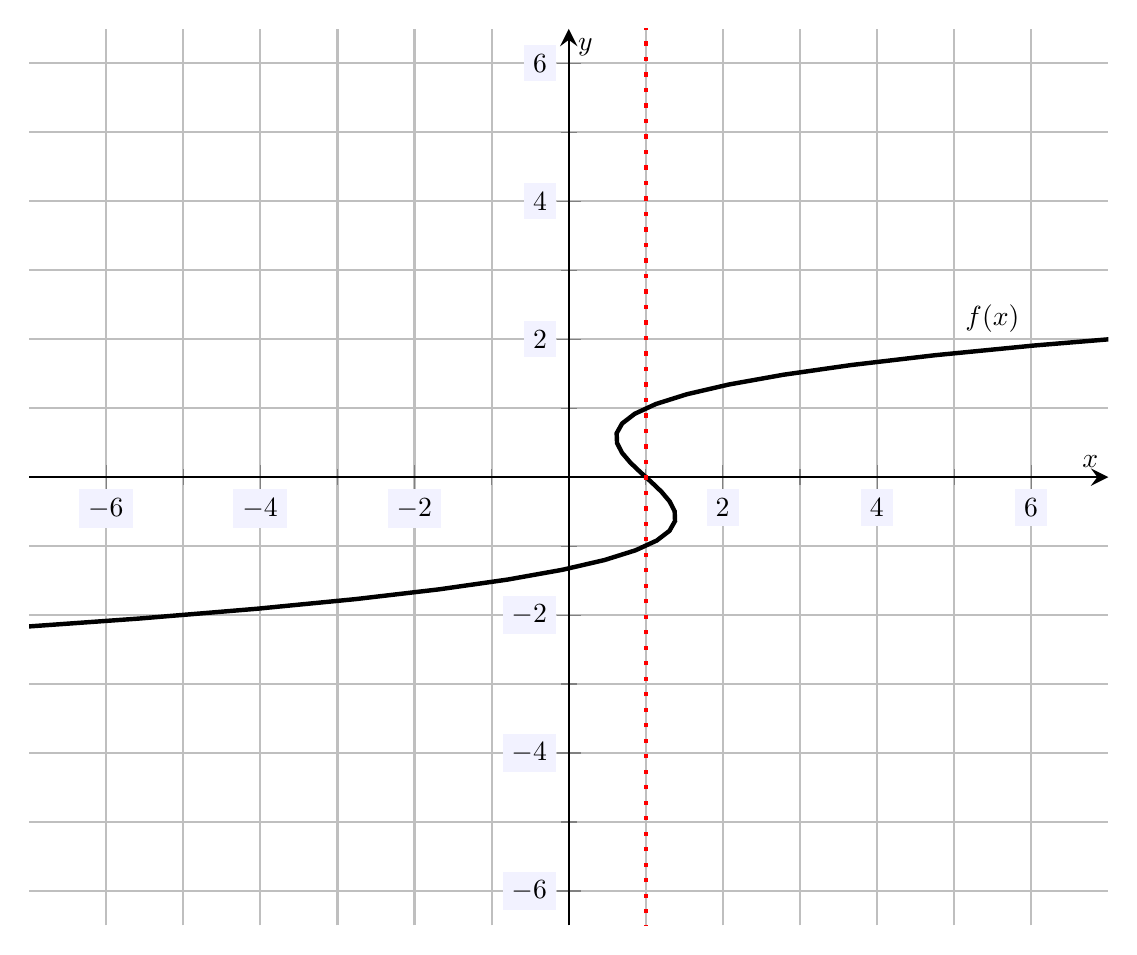
\begin{tikzpicture}[scale=2,every node/.style={scale=0.5}]
	\begin{axis}[
	grid=both,
	axis lines=middle,
	ticklabel style={fill=blue!5!white},
	xmin= -7, xmax=7,
	ymin= -6.5, ymax=6.5,
	xtick={-6,-4,-2,0,2,4,6},
	ytick={-6,-4,-2,0,2,4,6},
	minor tick = {-5,-3,...,5},
	xlabel=\(x\),ylabel=\(y\),
	]
	\node at (5.5,2.3) {$f(x)$};
	\addplot[thick, domain= -7:7, samples=100] ({x^3-x+1},{x});
	\addplot[red, dotted, thick, domain= -7:7] ({1},{x});
	\end{axis}
	\end{tikzpicture}
	}
	\] \pspace

\sol The relation plotted is not a function because this relation does not pass the vertical line test, i.e. not every vertical line intersects the relation $f(x)$ at most once. For instance, the vertical line at $x= 1$ intersects the relation $f(x)$ 3 times so that we do not know if $f(1)= -1$, $f(1)= 0$, or $f(1)= 1$, i.e. $f(1)$ is not well defined. 



\newpage



% Problem 3
\problem{10} Determine if the relations $f(x)$ and $g(x)$ shown below are functions. Explain why or why not. 
	\[
	\begin{aligned}
	f(x)&= 6.73 - 13.54x \\[0.3cm]
	g(x)&= \dfrac{6x - 5}{3x^2 + 1}
	\end{aligned}
	\] \pspace

\sol Both relations $f(x)$ and $g(x)$ are functions. For each input, there is only one possible output---the one obtained by `plugging in' for $x$ and following order of operations. 



\newpage




% Problem 
\problem{10} Suppose $f(x)$ is the function given below.
	\[
	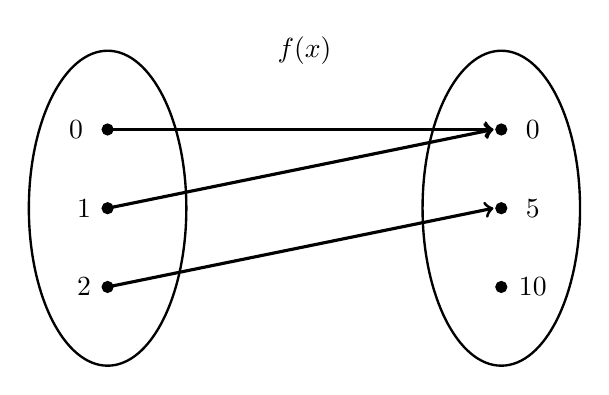
\begin{tikzpicture}
	\node at (2.5,2) {$f(x)$};
	% Ellipses
	\draw[line width=0.03cm] (0,0) circle (1 and 2);
	\draw[line width=0.03cm] (5,0) circle (1 and 2);
	
	% Nodes
	\draw[fill=black] (0,1) circle (0.07);
	\draw[fill=black] (0,0) circle (0.07);
	\draw[fill=black] (0,-1) circle (0.07);
	
	\draw[fill=black] (5,1) circle (0.07);
	\draw[fill=black] (5,0) circle (0.07);
	\draw[fill=black] (5,-1) circle (0.07);
	
	% Arrow
	\draw[line width=0.04cm,->] (0,1) -- (4.9,1);
	\draw[line width=0.04cm,->] (0,0) -- (4.9,1);
	\draw[line width=0.04cm,->] (0,-1) -- (4.9,0);
	
	% Labels
	\node at (-0.4,1) {$0$};
	\node at (-0.3,0) {$1$};
	\node at (-0.3,-1) {$2$};
	
	\node at (5.4,1) {$0$};
	\node at (5.4,0) {$5$};
	\node at (5.4,-1) {$10$};
	\end{tikzpicture}
	\]

\begin{enumerate}[(a)]
\item What is the domain of $f(x)$?
\item What is the codomain of $f(x)$?
\item What is the range of $f(x)$?
\end{enumerate} \pspace

\sol
\begin{enumerate}[(a)]
\item The domain for $f(x)$ is the set $\{ 0, 1, 2 \}$. \pspace

\item The codomain for $f(x)$ is the set $\{ 0, 5, 10 \}$. \pspace

\item The range of $f(x)$ is the set $\{ 0, 5 \}$. 
\end{enumerate}



\newpage



% Problem 
\problem{10} Determine whether the point $(2, -1)$ is on the graph of $f(x)= 2x^2 - 5x + 3$. Determine also whether the point $(1, 0)$ is on the graph of $f(x)$. For each, explain why or why not. \pspace

\sol If $(2, -1)$ is on the graph of $f(x)$, then it must be that $f(2)= -1$. However,
	\[
	f(2)= 2(2^2) - 5(2) + 3= 2(4) - 5(2) + 3= 8 - 10 + 3= -2 + 3= 1
	\]
Therefore, $(2, -1)$ is not on the graph of $f(x)$, rather $(2, 1)$ is on the graph of $f(x)$. \pspace

Similarly, to determine whether the point $(1, 0)$ is on the graph of $f(x)$, we check whether $f(1)= 0$:
	\[
	f(1)= 2(1^2) - 5(1) + 3= 2(1) - 5(1) + 3= 2 - 5 + 3= -3 + 3= 0
	\]
Therefore, $(1, 0)$ is on the graph of $f(x)$. 



\newpage



% Problem 
\problem{10} Suppose $f(x)$ and $g(x)$ are the functions given below. 
        \begin{table}[!ht]
        \centering
        \begin{tabular}{| c || c | c | c | c | c | c | c |} \hline
	$x$ & $-3$ & $-2$ & $-1$ & $\phantom{-}0$ & $\phantom{-}1$ & $\phantom{-}2$ & $\phantom{-}3$ \\ \hline
	$f(x)$ & $3$ & $-2$ & $1$ & $6$ & $4$ & $-7$ & $0$ \\ \hline
	$g(x)$ & $2$ & $1$ & $0$ & $3$ & $-5$ & $-5$ & $-4$ \\ \hline
	$h(x)$ & $0$ & $1$ & $0$ & $3$ & $0$ & $-1$ & $6$ \\ \hline
        \end{tabular}
        \end{table}

Compute the following: \pspace
        \begin{enumerate}[(a)]
        \item $(f + g)(1)= f(1) + g(1)= 4 + (-5)= -1$ \vfill
        \item $(f - g)(-2)= f(-2) - g(-2)= -2 - 1= -3$ \vfill
        \item $(-2h)(3)= -2h(3)= -2 \cdot 6= -12$ \vfill
        \item $\left(\dfrac{h}{g}\right)(0)= \dfrac{h(0)}{g(0)}= \dfrac{3}{3}= 1$ \vfill
        \item $f(0)\, h(-2)= 6 \cdot 1= 6$ \vfill
        \item $f(2 - h(0))= f(2 - 3)= f(-1)= 1$ \vfill
        \item $(f \circ g)(0)= f(g(0))= f(3)= 0$ \vfill
        \item $(g \circ h)(2)= g(h(2))= g(-1)= 0$ \vfill
        \item $(f \circ g \circ h)(1)= f(g(h(1)))= f(g(0))= f(3)= 0$ \vfill
        \item $(h \circ g)(-2)= h(g(-2))= h(1)= 0$
        \end{enumerate} \pspace



\newpage



% Problem 
\problem{10} Suppose $f(x)$ and $g(x)$ are the functions given below. 
	\[
	\begin{aligned}
	f(x)&= 4 - 3x \\[0.3cm]
	g(x)&= x^2 - x + 4
	\end{aligned}
	\]

Compute the following: \pspace
\begin{enumerate}[(a)]
\item $f(2)= 4 - 3(2)= 4 - 6= -2$ \vfill
\item $g(1)= 1^2 - 1 + 4= 1 - 1 + 4= 4$ \vfill
\item $3f(1) - g(2)= 3(4 - 3 \cdot 1) - (2^2 - 2 + 4)= 3(4 - 3) - (4 - 2 + 4)= 3(1) - (2 + 4)= 3 - 6= -3$ \vfill
\item $f(x) - g(x)= (4 - 3x) - (x^2 - x + 4)= 4 - 3x - x^2 + x - 4= -x^2 - 2x$ \vfill
\item $f(x) \, g(x)= (4 - 3x)(x^2 - x + 4)= 4x^2 - 4x + 16 - 3x^3 + 3x^2 - 12x= -3x^3 + 7x^2 - 16x + 16$ \vfill
\item $\left( \dfrac{f}{g} \right)(x)= \dfrac{4 - 3x}{x^2 - x + 4}$ \vfill
\item $(f \circ g)(0)= f(g(0))= f(0^2 - 0 + 4)= f(4)= 4 - 3(4)= 4 - 12= -8$ \vfill
\item $(g \circ f)(1)= g(f(1))= g(4 - 3 \cdot 1)= g(1)= 1^2 - 1 + 4= 4$ \vfill
\item $(f \circ g)(x)= f(g(x))= f(x^2 - x + 4)= 4 - 3(x^2 - x + 4)= 4 - 3x^2 + 3x - 12= -3x^2 + 3x - 8$ \vfill
\item $(g \circ f)(x)= g(f(x))= g(4 - 3x)= (4 - 3x)^2 - (4 - 3x) + 4= 16 + 9x^2 - 24x - 4 + 3x + 4= 9x^2 - 21x + 16$ \vfill
\end{enumerate} \pspace



\newpage



% Problem 
\problem{10} Given the graph of $f(x)$ below, determine whether $f(x)$ has an inverse function. Explain why or why not. 
	\[
	\fbox{
	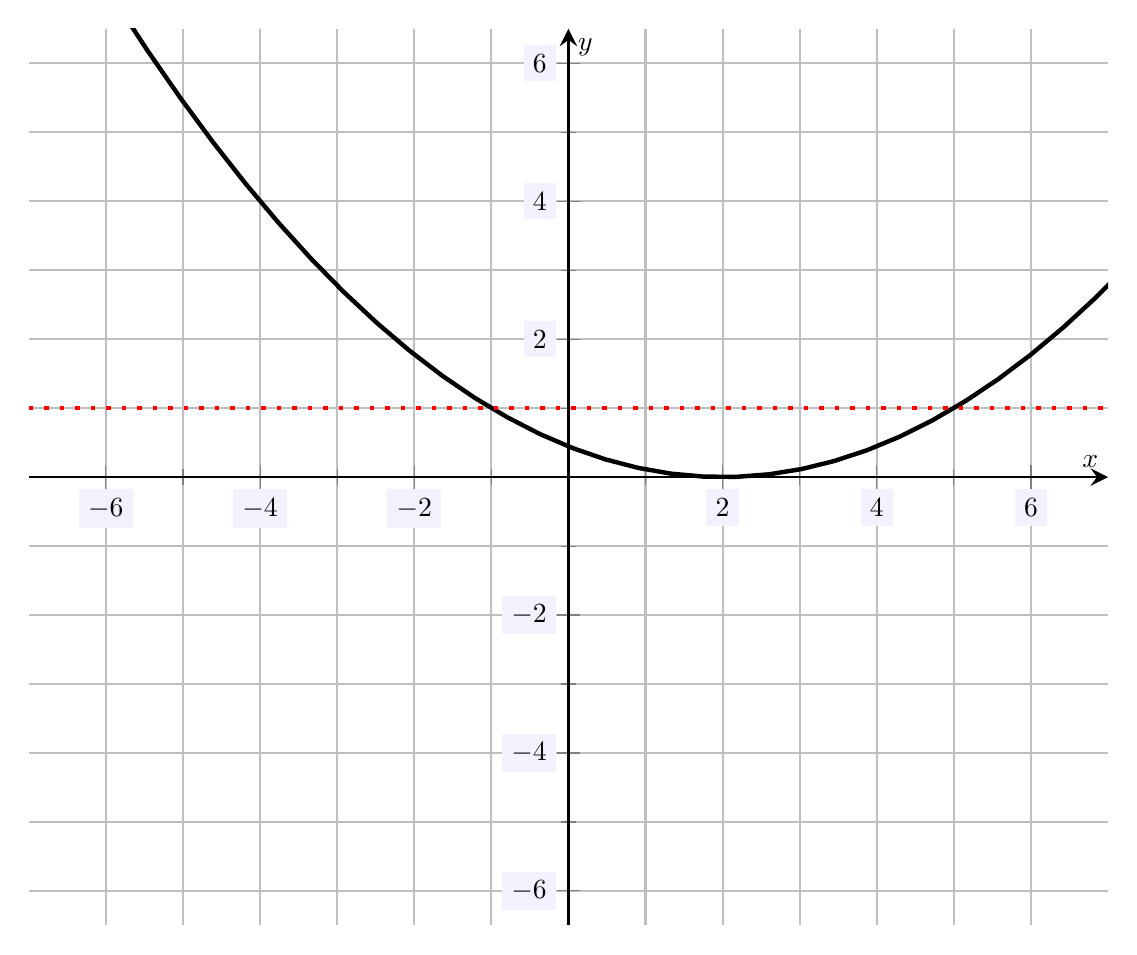
\begin{tikzpicture}[scale=2,every node/.style={scale=0.5}]
	\begin{axis}[
	grid=both,
	axis lines=middle,
	ticklabel style={fill=blue!5!white},
	xmin= -7, xmax=7,
	ymin= -6.5, ymax=6.5,
	xtick={-6,-4,-2,0,2,4,6},
	ytick={-6,-4,-2,0,2,4,6},
	minor tick = {-5,-3,...,5},
	xlabel=\(x\),ylabel=\(y\),
	]
	\addplot[thick, domain= -7:7,samples=100] ({3*x-1},{x^2-2*x+1});
	\addplot[red, dotted, thick, domain= -7:7] ({x},{1});
	\end{axis}
	\end{tikzpicture}
	}
	\] \pspace

\sol The function, $f(x)$, plotted above does not have an inverse function because it fails the horizontal line test, i.e. not every horizontal line intersects the function in at most one point. For instance, the horizontal line at $y= 1$ intersects the function at $(-1, 1)$ and $f(5,1)$. 



\newpage



% Problem 
\problem{10} Given the graph of $f(x)$, sketch the function $f^{-1}(x)$. Determine also $f^{-1}(1)$ and $f^{-1}(2)$. 
	\[
	\fbox{
	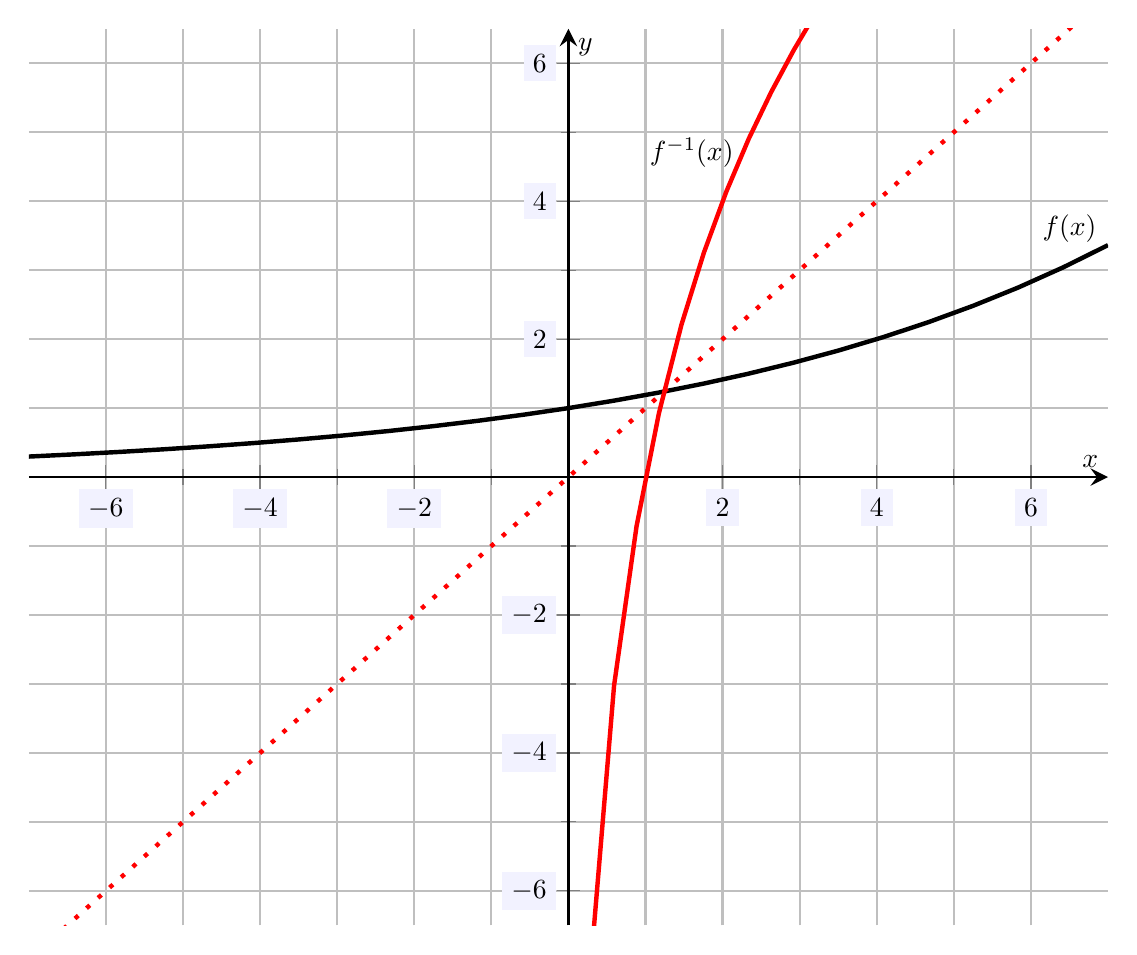
\begin{tikzpicture}[scale=2,every node/.style={scale=0.5}]
	\begin{axis}[
	grid=both,
	axis lines=middle,
	ticklabel style={fill=blue!5!white},
	xmin= -7, xmax=7,
	ymin= -6.5, ymax=6.5,
	xtick={-6,-4,-2,0,2,4,6},
	ytick={-6,-4,-2,0,2,4,6},
	minor tick = {-5,-3,...,5},
	xlabel=\(x\),ylabel=\(y\),
	]
	\node at (6.5,3.6) {$f(x)$};
	\addplot[thick, domain= -7:7] {2^(x/4)};
	\node at (1.6,4.7) {$f^{-1}(x)$};
	\addplot[red, thick, domain= 0.01:7] {4*ln(x)/ln(2)};
	\addplot[red, thick, dotted, domain= -7:7] {x};
	\end{axis}
	\end{tikzpicture}
	}
	\] \pspace

\sol If a function $f(x)$ has an inverse function, the graph of $f^{-1}(x)$ is the reflection of $f(x)$ through the line $y= x$. From this plot, we can see that $f^{-1}(1)= 0$ and $f^{-1}(2)= 4$. Alternatively, we can see from the graph of $f(x)$ that $f(x)= 1$ when $x= 0$ (the horizontal line at $y= 1$ intersects the curve at the point $(0, 1)$) so that $f^{-1}(1)= 0$. Similarly, we can see from the graph of $f(x)$ that $f(x)= 2$ when $x= 4$ (the horizontal line at $y= 2$ intersects the curve at the point $(4, 2)$) so that $f^{-1}(2)= 4$.


\end{document}